\documentclass[a4paper,12pt]{article}
\usepackage[utf8]{inputenc}
\usepackage[T1]{fontenc}
\usepackage[spanish]{babel}
\usepackage{anysize}
\usepackage{graphicx}
\marginsize{25mm}{25mm}{25mm}{25mm}

\title{Why do animals make better choices in patch-leaving problems?}
\author{David W. Stephens, Aimee S. Dunlap}
\date{2009}

\begin{document}

{\scshape\bfseries \maketitle}

Los animales suelen elegir de manera impulsiva cuando las alternativas que se les ofrecen varían en tiempo y magnitud. Se ha intentado explicar mediante descuento (la demora implica incertidumbre sobre la obtención del reforzador), pero el grupo de Stephens ha buscado explicar mediante lo que llaman ``racionalidad ecológica'': la idea de que las reglas de decisión impulsivas existen dado que se desempeñan bien en la naturaleza.

Se ha mostrado que los {\itshape blue jays} muestran impulsividad en el procedimiento clásico de descuento, pero maximizan en una situación de abandono de parche en la cual, tras recibir una recompensa, pueden abandonar y comenzar de nuevo el ensayo, o permanecer y recibir una segunda recompensa. Se intentará demostrar que la racionalidad ecológica puede explicar ambos fenómenos.

{\bfseries Patch and self control in standard form.} 

En el procedimiento de impulsividad se entregan recompensas de distintas magnitudes a distintos tiempos con la misma demora. En el de parches se entrega una recompensa tras una demora larga en la opción de abandonar, y en la opción de permanecer se entrega primero una recompensa adicional tras una demora pequeña, seguida de una segunda recompensa con propiedades idénticas a las de la otra alternativa (figura 1).

\begin{figure}[ht]
	\begin{center}
		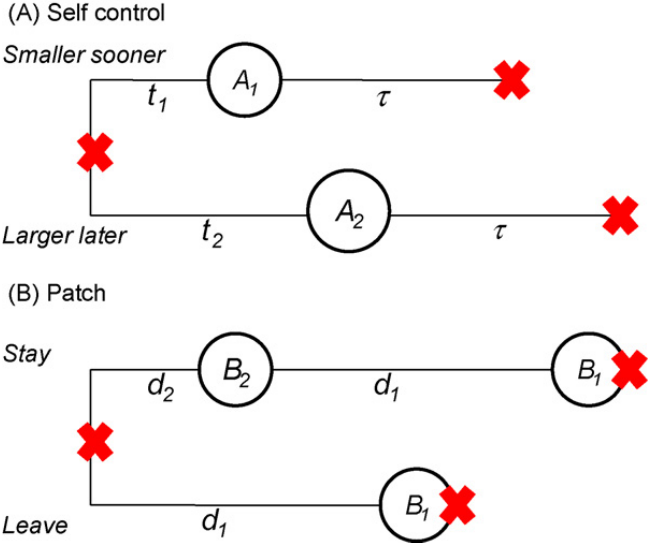
\includegraphics[scale=0.5]{Stephens2009(1).png}
		\caption{Representación estandarizada de ambos procedimientos.}
	\end{center}
\end{figure}

{\bfseries The algebra of impulsivity.}

Una forma de conceptualizar la elección racional es mediante la ganancia a largo plazo: la recompensa dividida entre el tiempo hasta la siguiente oportunidad de elección. Para la situación de autocontrol se compara $\frac{A_{1}}{\tau + t_{1}}$ con $\frac{A_{2}}{\tau + t_{2}}$. Para la de parche se calcula $\frac{B_{1} + B_{2}}{d_{1} + d_{2}}$ para la opción de permanecer, y $\frac{B_{1}}{d_{1}}$ para la de abandonar.

Un modelo distinto de ganancias a corto plazo ignora lo intervalos entre ensayos y solo considera los tiempos pre-reforzamiento, por lo que en el procedimiento de autocontrol se compararía $\frac{A_{1}}{t_{1}}$ con $\frac{A_{2}}{t_{2}}$, lo que lleva a impulsividad si el ITT es largo. En la situación de parche se compararía $\frac{B_{1}}{d_{1}}$ con $\frac{B_{2}}{d_{2}}$. Algebraicamente esta ecuación es igual a la del modelo a largo plazo, con lo que los animales no pueden hacer elecciones impulsivas en el procedimiento de parche.

La idea de la racionalidad biológica es que los animales emplean el modelo a corto plazo porque la naturaleza tiende a reducir o eliminar los costos de las elecciones impulsivas. El grupo de Stephens ha explorado esta idea en artículos previos. En uno de ellos crearon situaciones de parche y autocontrol que eran equivalentes en el corto plazo en lugar de el largo plazo. Sus resultados contradijeron la idea de que la regla de corto plazo puede explicar la conducta en ambas situaciones. Su segundo experimento mostró que los sujetos toman al intervalo entre ensayos (antes de ``elegir'' interactuar con el parche) y a la primera demora a la comida como una demora combinada.

Este estudio replicará primero el hallazgo de que la regla a corto plazo no puede explicar la conducta de ambas situaciones. Después tratará de responder si la segunda entrega de comida en la opción de permanecer en la situación de parche puede explicar las diferencias observadas en la conducta entre los dos procedimientos.

{\bfseries Rationale.}

Habrá tres condiciones: situación de parche estándar, de autocontrol estándar, y de autocontrol+. En autocontrol+ se agregará una entrega adicional de comida en momentos y cantidades paralelos a la condición de parche (figura 2)

\begin{figure}[ht]
	\begin{center}
		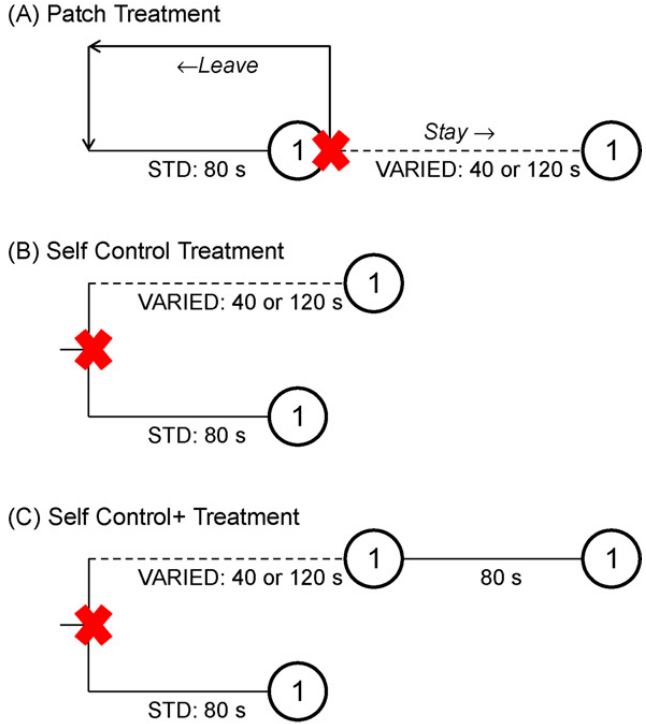
\includegraphics[scale=0.5]{Stephens2009(2).png}
		\caption{Los tres tratamientos del experimento.}
	\end{center}
\end{figure}

Este experimento tiene el propósito de determinar si la segunda entrega de reforzamiento determina la elección. Se varió la demora asociada con la alternativa de permanecer y sus análogos en la otra situación entre dos valores elegidos para que uno fuese corto (y por lo tanto elegido bajo casi cualquier modelo económico) y otro largo (prediciendo que será rechazado). Es un diseño factorial con tres niveles de situación y dos de demora.

El modelo de corto plazo hace predicciones idénticas para las tres condiciones dado que las demoras  magnitudes asociadas con la primera entrega de comida son iguales. Si hay sensibilidad a las consecuencias a largo plazo, las condiciones de autocontrol y autocontrol+ deberían diferir. Si la hipótesis de la segunda entrega de comida es correcta se esperaría comportamiento idéntico en autocontrol+ y en parche.

{\bfseries Methods}

Los sujetos elegían parándose en perchas de elección. Se trató de una economía cerrada en la que pasaban 23 horas al día en el aparato.

Cada sujeto experimentó los 6 tratamientos (3 situaciones $\times$ 2 demoras) en orden aleatorio. Se buscó probar tanto la hipótesis de segunda entrega de reforzamiento como la de corto plazo.

Se analiza la frecuencia con que los sujetos escogen la alternativa experimentalmente variada ({\itshape i.e.,} la que puede tener demora de 40 o 120s). La alternativa complementaria será llamada estándar. Se espera que los sujetos acepten la alternativa variada cuando su demora es corta, y la rechacen cuando es larga (la demora solo varió entre condiciones, nunca intra).

En la situación de parche las aves esperaban en una percha trasera durante un ITT $\theta$ tras el cual se encendía alguna de las luces de las perchas frontales aleatoriamente. El ave podía volar hacia la percha iluminada y recibir comida, y luego tenía la opción de permanecer en ella por la demora especificada por el programa (señalada por el color de la luz) o regresar a la percha trasera para comenzar un nuevo ITT.

En la situación de autocontrol las aves ocupaban la percha trasera seguido de lo cual se encendían ambas perchas frontales. Un color (no posición) se asociaba con la opción experimentalmente variada, y el otro con la estándar.El ave elegía volando hacia la percha correspondiente y eso comenzaba la demora. A diferencia de otras situaciones de autocontrol, aquí el ITT fue brevísimo (3 s) y las alternativas no diferían en magnitud, sino solo en demora.

En autocontrol+ la situación era idéntica salvo por la entrega de un pellet adicional 80 segundos después del primero. No se podía abandonar esta segunda entrega.

La tarea se dividió en bloques de 32 ensayos de los cuales los primeros 12 eran forzados. Entre condiciones se hizo un procedimiento de {\itshape titration} con el propósito de regresar a los sujetos a la indiferencia antes de cada cambio de condición. En este procedimiento se variaba la demora de la alternativa variada en función de las elecciones de los sujetos para llevarlos a indiferencia.

Para detectar efectos de adquisición se dividieron los 900 ensayos toados en cuenta en bloques de 300. El análisis entonces puede verse como 3$\times$2$\times$3.

{\bfseries Results}

Cualitativamente de acuerdo con lo esperado, las aves eligieron con más frecuencia la opción variada cuando su demora era corta que cuando era larga. Ejecutaron de la forma económicamente mejor en la situación de parches y peor en la de autocontrol+.

Hubo una interacción significativa entre situación, demora y bloque, con lo que el efecto de la demora depende tanto del patrón de adquisición como de las diferencias en la situación.

Si se analiza solamente el bloque final se observa que la ejecución difirió entre situaciones en la demora de 120 segundos: los sujetos evitaron confiablemente esa opción en la situación de parche, como se esperaba, pero tuvieron un desempeño pobre, cercano al 50\%, en autocontrol+. En autocontrol su desempeño fue intermedio.

{\itshape Programmed vs realized delays.} Aunque las demoras eran idénticas en todos los procedimientos, es posible que ciertos procedimientos hicieran a los animales escoger más pronto que otros, lo que explicaría en parte las diferencias observadas. Para evaluar esto se calculó la diferencia entre demoras programadas y realizadas en función de la situación, la elección realizada, y la demora. Esto reveló dos efectos significativos: las demoras programadas y realizadas difieren más cuando los sujetos eligen la opción más demorada (lo que no puede explicar las diferencias en elección), y las demoras programadas y realizadas difieren entre las tres situaciones de elección. La diferencia es mínima en autocontrol y más en parche. Se concluye que aunque hay diferencias intrigantes en las demoras, no están relacionadas con los resultados observados.

{\bfseries Discussion}

Se probó la hipótesis de que el procedimiento de parche lleva a elegir la alternativa grande demorada debido a la entrega de un segundo reforzador, y la aplicabilidad de una regla de decisión de corto plazo en situaciones de autocontrol y de parche.

Hay cuatro resultados clave:

\begin{enumerate}
	\item No se apoya la hipótesis de la segunda entrega dado que la situación de autocontrol+ difirió más de la de parche.
	\item La regla de corto plazo no puede explicar la conducta observada debido a que las tres situaciones ofrecieron recompensas idénticas en el corto plazo y aun así se encontraron diferencias.
	\item Se replican resultados previos que indican que los animales ejecutan mejor en la situación de parche.
	\item La comparación de autocontrol con autocontrol+ indica que la segunda entrega sí puede influir en la elección. Los sujetos elegían la opción variada más a menudo cuando era seguida de una entrega adicional de comida, pero solo con la demora larga.
\end{enumerate}

Se podría argumentar que los animales utilizan reglas de elección fundamentalmente distintas en las dos situaciones, lo que haría irrelevante a la aproximación de la racionalidad ecológica a la impulsividad. Una alternativa sería que hay una regla común aun no identificada en ambas situaciones.

{\itshape Limitations}

Aunque los modelos sugieren que la situación de parche es similar a una de autocontrol sin ITT, se utilizó un intervalo de 3 s en las condiciones de autocontrol, por lo que en teoría no se puede esperar la misma conducta. Pero en todo caso, se debería haber encontrado conducta idéntica entre parche y autocontrol+, pero las condiciones más diferentes fueron parche y autocontrol+.

Estos resultados no indican que la segunda entrega no sea importante en la situación de parche, solo que no explica las diferencias entre parche y autocontrol.

Finalmente, se puede argumentar que las situaciones son sumamente simples y no representan a situaciones reales.

{\itshape Where next?}

Dado que los procedimientos de parche y autocontrol+ crean elecciones con idéntico tiempo y consecuencias, ningún modelo actual puede explicar los resultados. Para explicarlos se sugieren varias posibilidades. Primero, aunque las consecuencias eran idénticas los animales pudieron experimentar consecuencias distintas en alguna forma que sesgó su conducta. Segundo, en la situación de parche las alternativas difieren en el costo de respuesta (quedarse {\itshape vs.} abandonar), mientras que en autocontrol ambas alternativas tienen el mismo costo. Esta diferencia puede llevar a distintos patrones de elección.

{\itshape Where does this leave ecological rationality?}

Es incierto.

La racionalidad ecológica aplica en cualquier situación en la cual los dominios de selección y prueba sean distintos. Quedan preguntas sobre cómo debería proceder un programa de investigación basado en esta idea. Es necesaria una teoría que pueda establecer relaciones entre el dominio de selección, con su infinidad de dimensiones, y los posibles dominios de prueba. Además, el argumento de la racionalidad ecológica es muy fácil como escape debido a que se le puede atribuir virtualmente cualquier desviación de las expectativas económicas.




\end{document}
